\documentclass{beamer}
\usepackage[utf8]{inputenc}

\title{Dinamik Programlama ile Antik Yazılar Üzerinde Çalışmak}
\author{Kaan Eraslan}
\date{\today}

\begin{document}

\note{Butun resimler wikimedia'dan alinmistir, sunumdaki slidelara da benim yayin için kullandigim depodan ulasabilirsiniz.}
\maketitle
\begin{frame}{Yapay Zeka Uygulama Alani Olarak Eski Tarih}
\center Eski Oldu da Ne Oldu ?
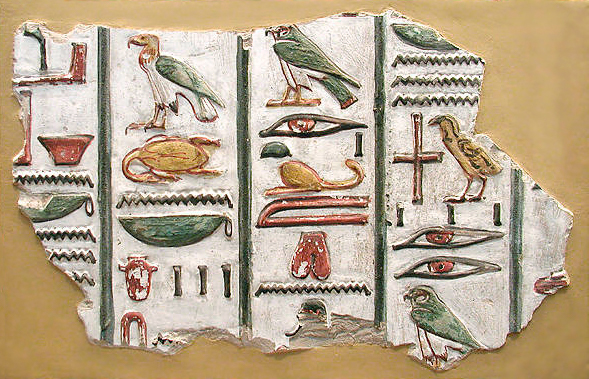
\includegraphics[width=\linewidth, keepaspectratio]{hieoroglyph.jpg}
    
\end{frame}
\note{
\begin{itemize}
    \item özünde bir farklilik yok
    \item veri sayisi az
    \item veri üretimi çok mesakatli
    \begin{itemize}
        \item Uretim sureci uzmanlik gerektiriyor: Araba ve 3. yuzyildaki sigma karakterini siniflamak
        \item Çok sıkıcı bir iş.
        \item Biz o kadar da kesin bilmiyoruz 3. yuzyildan mi 5. yuzyildan mi, arkeometrik metotlar 1 herseye uygulanmiyor, 2 bunlarla tarihlendirme yapilirken de mevcut tarihi bilgiden faydalaniliyor.
    \end{itemize}
\end{itemize}
}

\begin{frame}{Uygulama Alanlari Nelerdir ?}
\center Şu anda neye uygulanıyorsa o
\includegraphics[width=\linewidth, keepaspectratio]{zekatarih.jpg}

\end{frame}

\note{
Yapay zekanin standart 3 alt alaninda gelistirilen teknolojiler uygulanabilir
\begin{itemize}
    \item Takviyeli ögrenim: Tarihi olgularin simulasyonu: Ya bu adamlar bu piramitleri nasil yapmis ? Piramit te bulunan tas ve yazili duvar miktari, taslarin çikarildigi yer, isçilerin kapasiteleri, ve piramidin yapim suresi goz onune alinarak olusturulabilir.
    \item Etiketli ögrenim: Supervised Learning,
    Elimde 1000 tane M.Ö 350'den eski yunanca metin var, 1001'inci eski yunanca metinde acaba M.Ö 350'den mi.
    \item Etiketsiz örengim: Unsupervised Learning,
    Ya su 500 heykelden bazilari sahte galiba (outlier detection) 
\end{itemize}
}

\begin{frame}{Zorluklar}
\begin{center}
    Her Sey El Yapimi, Biyolojik ve Tam Bugday

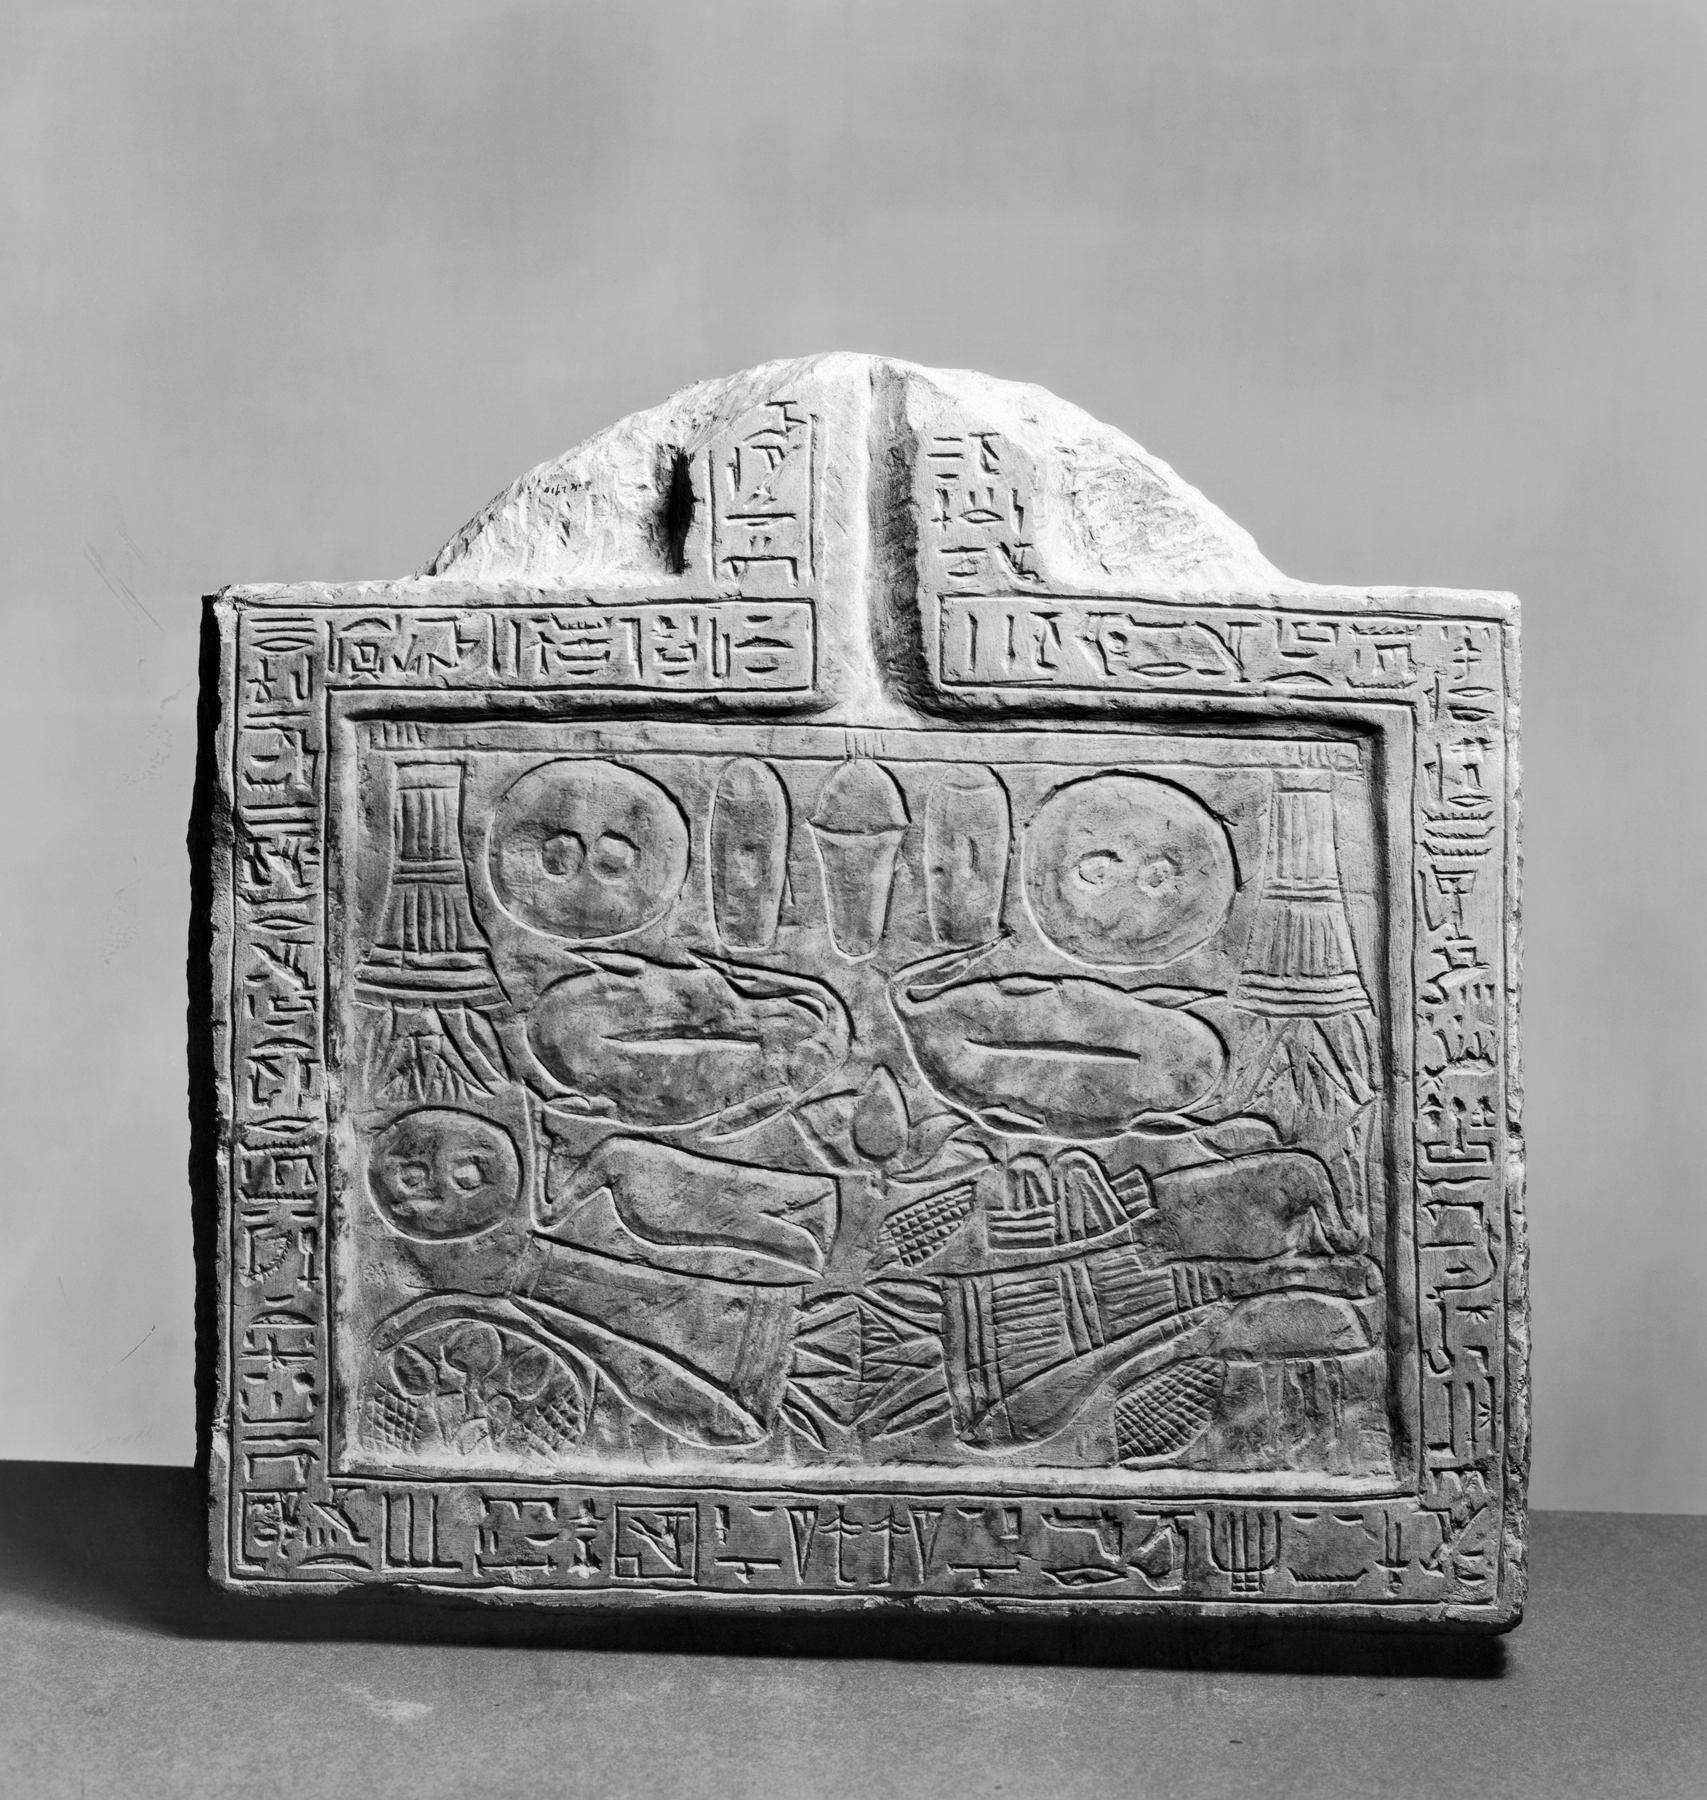
\includegraphics[scale=0.5,keepaspectratio]{offeringtable.jpg}
\end{center}
\end{frame}

\note{
Zorluklar:
\begin{itemize}
    \item Özellikle Matbaa öncesi dönemler de yaz yazmak sinai bir faaliyet. Iyi ayakkabi yapmak gibi yani.
    \item Traktor filan yok, her sey el ile yapiliyor dolayisiyla ham verinin standartlari çok esnek. 
    Ayni kisi ayni tipte vazoyu fabrikasyon yapmiyor, çok benzer sekilde yapiyor vs ama makine yapmis gibi olmuyor tabi.
\end{itemize}
}
\begin{frame}{Neye Ihtiyaç var ?}
\center Temiz veri

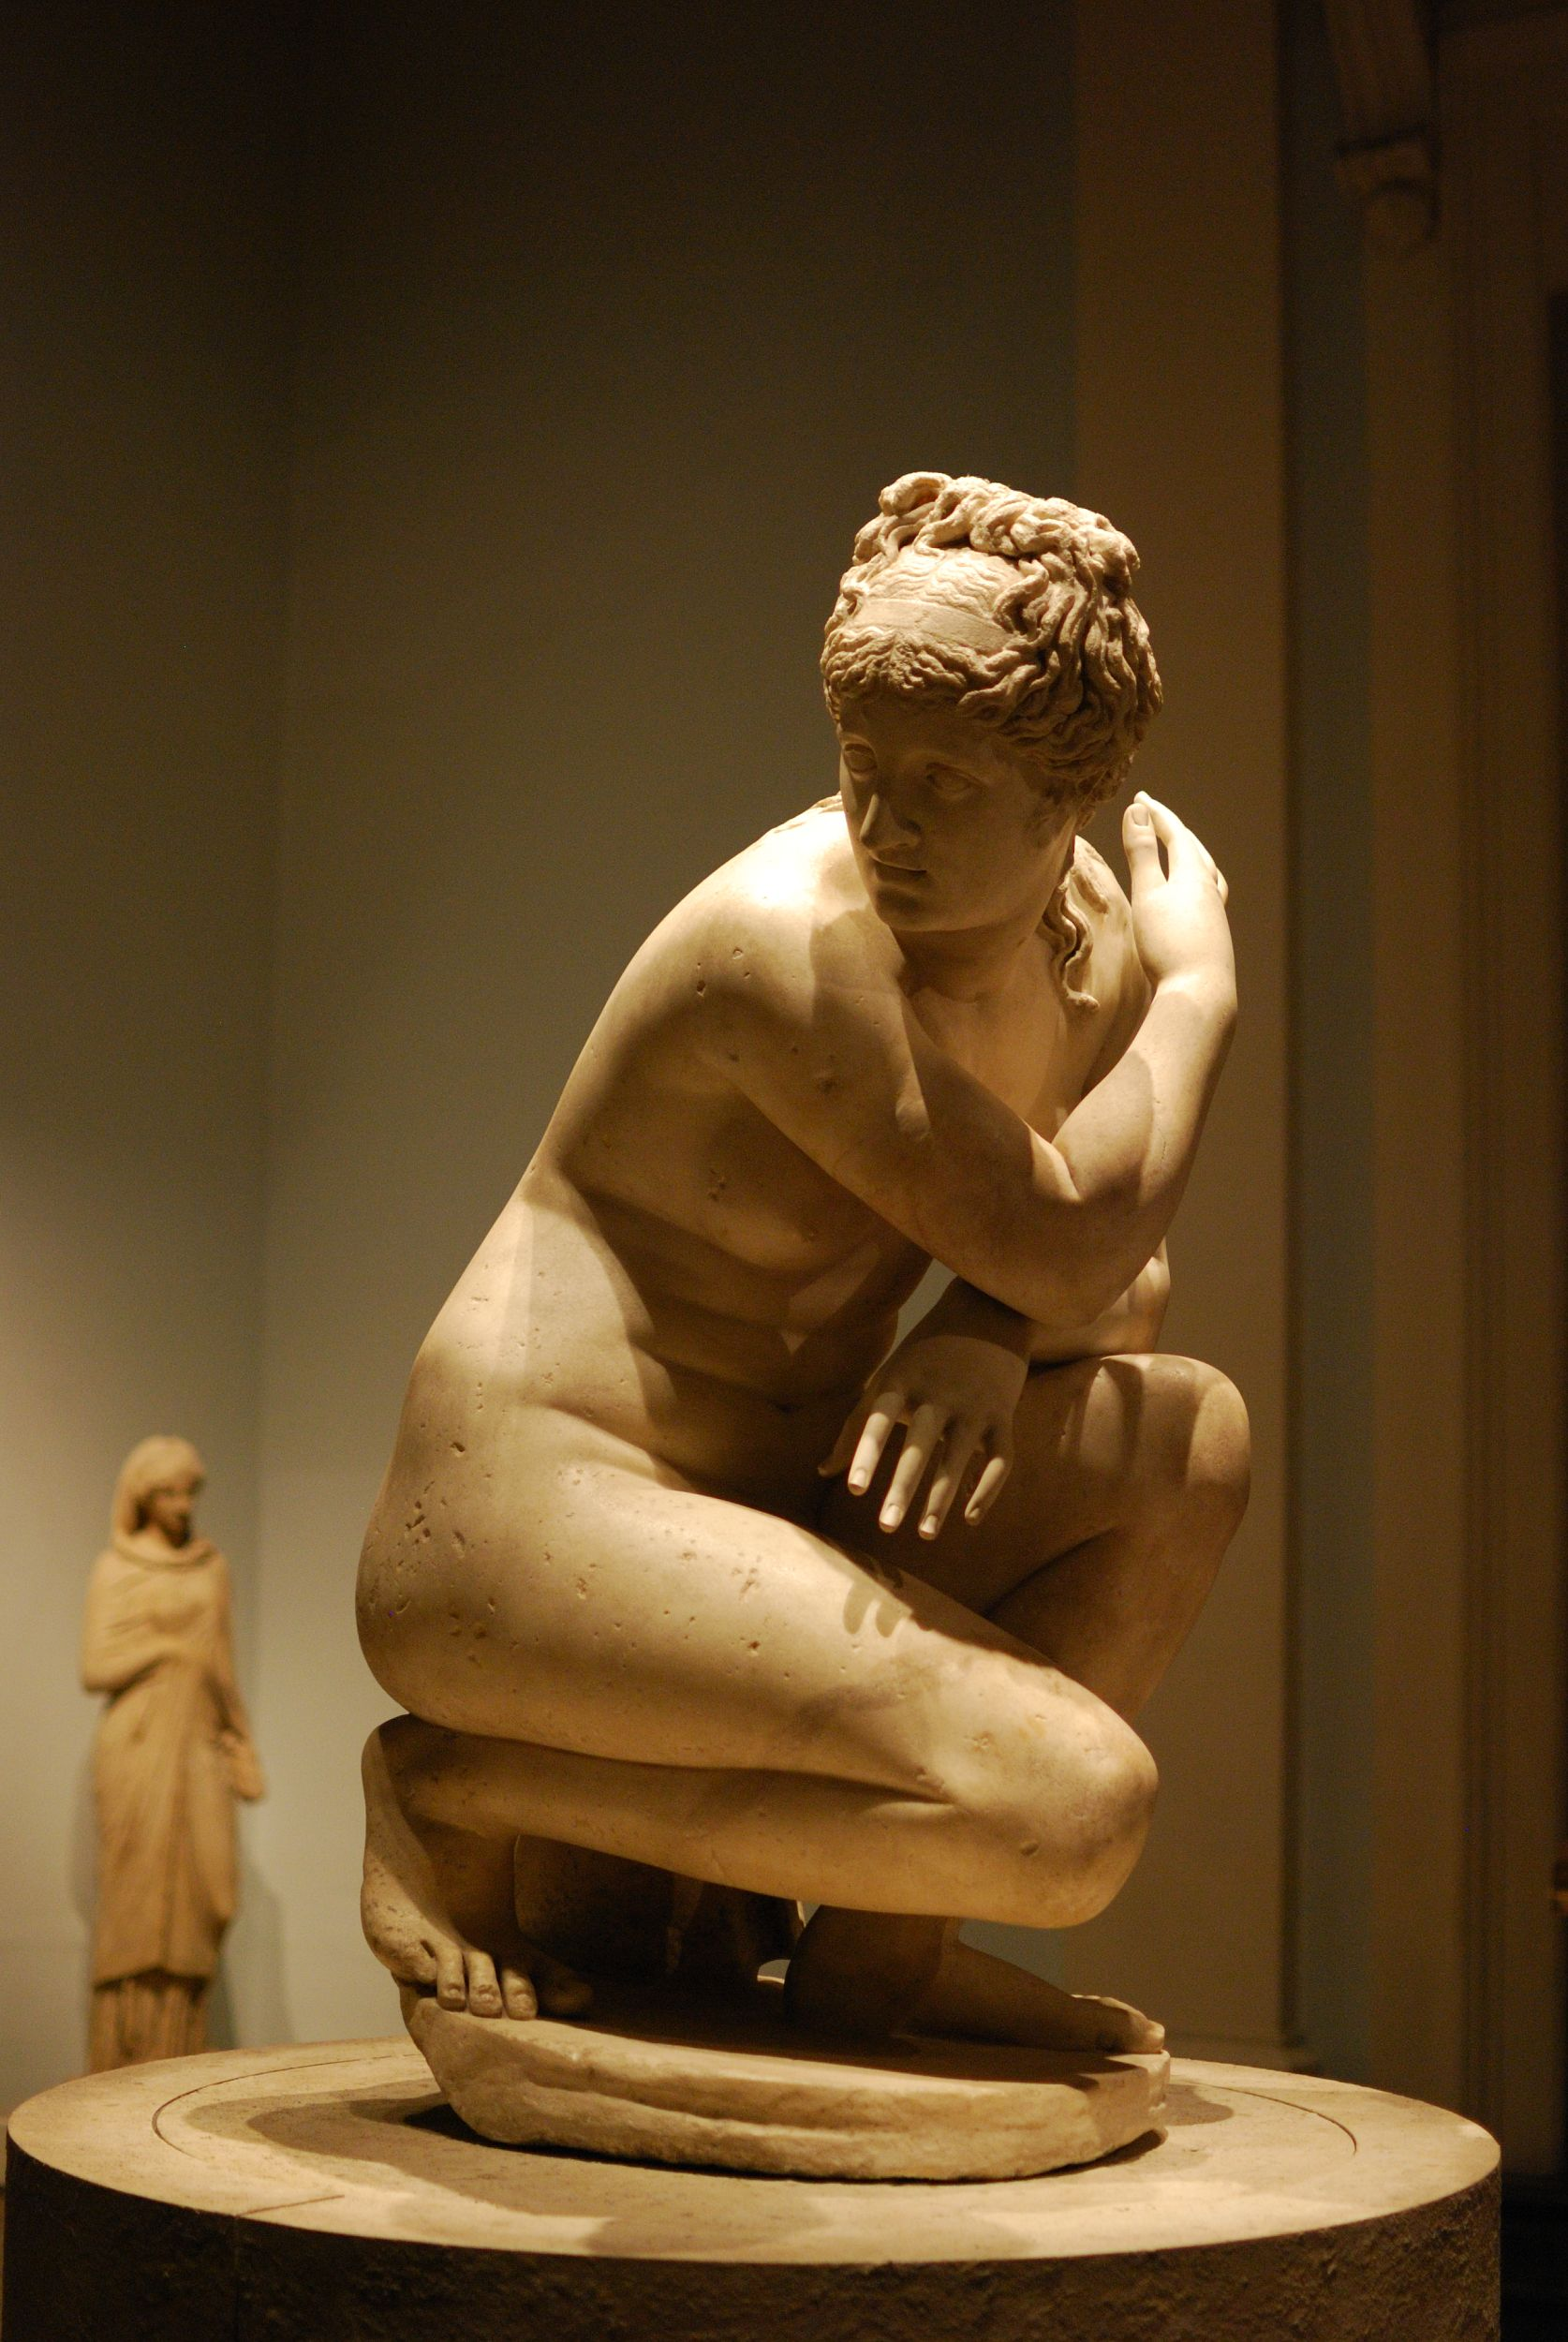
\includegraphics[keepaspectratio, scale=0.45]{afroditebath.jpg}    
\end{frame}
\note{
Standart yoksa ogrenme yok, veri temizligi veya temiz uretilmis veri sart.
Temiz veri uretimi elle mumkun degil, ya da genisletilebilir degil. 3 kisinin becerebildigi bir isi genel çozum diye savunmamnin bir manasi yok.
Dolayisiyla bu veri uretim surecine bir boru hatti ile otomatiklestirilebilen bir protokol ile cevap verilmesi gerekiyor.
}
\begin{frame}{Resim Siniflamak için Veri Uretimi}

\center Bir yerden baslamak lazim.

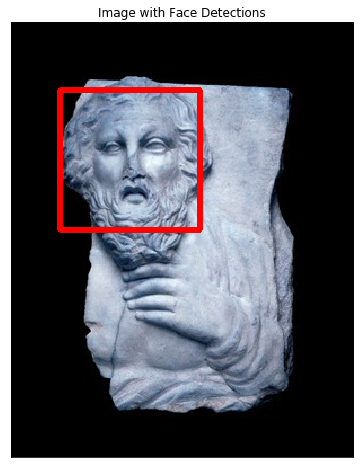
\includegraphics[scale=0.45]{statueFace1.png}
\end{frame}

\begin{frame}{Satir, Sutun, ve Enerji}
\center Dinamik Programlama ile butun bu islerin alakasi
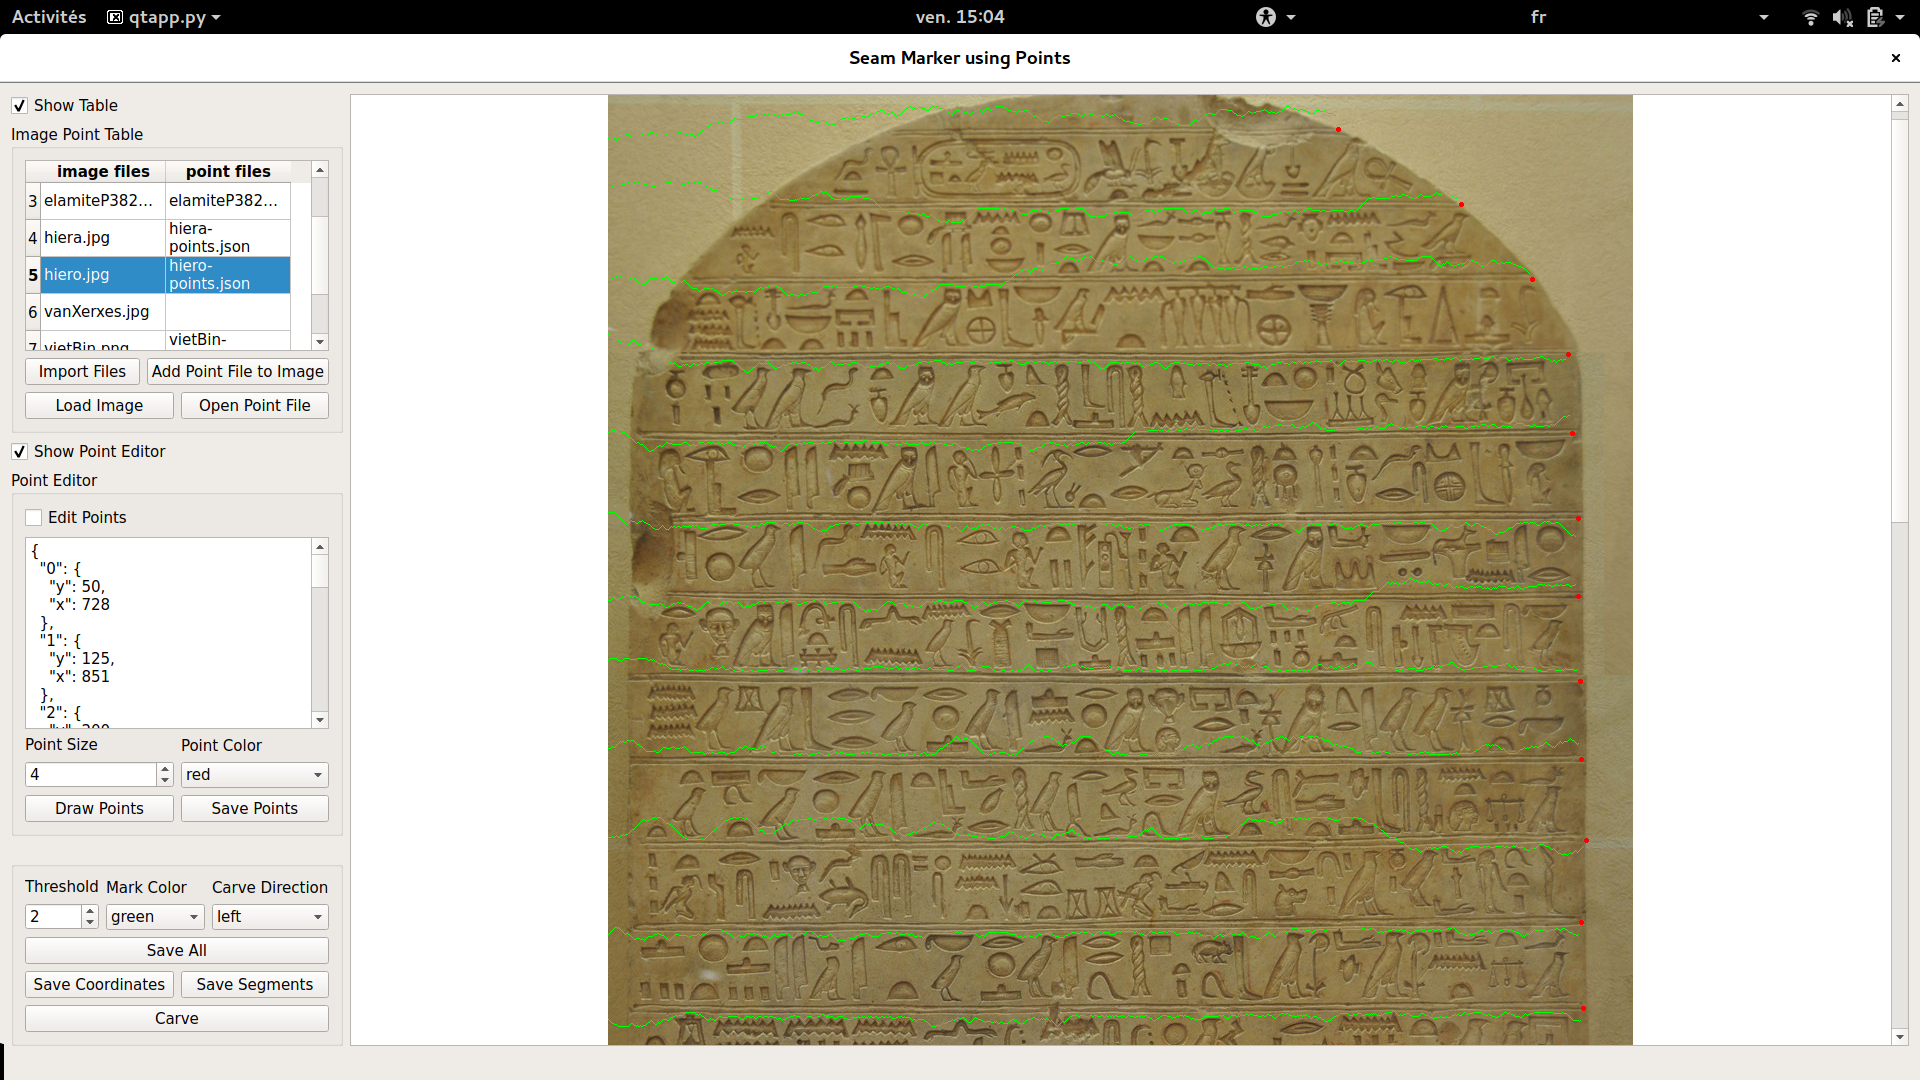
\includegraphics[scale=0.2]{SeamMarkerHiero.png}
\end{frame}
\note{
Satir, sutun nedir ? Ayiricidirlar.
Neyi ayirirlar ? Yazilari. Yazilar nedir ? Ecis bucus sekiller. Ayirici o halde ecis bucus olmayandir. Ayirici gorece homojendir. Enerjiyi kabaca renk turevi diye tarif edelim, dolayisiyla homojen alanlar, yani ayiricilar sifira yakin olurlar, ecis bucusler (Allah'a yakin olsunlar!), daha yuksek olurlar. O halde siradan toplasak, ayiricilarin aldigi deger, ecis bucuslerden daha dusuk olacaktir. Dinamik programlama bize en dusugunu bulacak sekilde siradan toplamamizda yardimci oluyor.
}
\begin{frame}{Kanal Gosterme (Seam Marking)}
Algoritmanin Genel Görünümü:
\begin{enumerate}
    \item Resmi matrise çevir
    \item Her pikselin enerjisini hesapla
    \item Dusuk enerji kanallarini hesapla
    \item En dusuk enerji kanalini isaretle
\end{enumerate}
\end{frame}

\begin{frame}{Numpy'da Görelim}
Kaynak Kodu Keyfi
\includegraphics[scale=0.05]{keyfi.jpg}

\end{frame}

\end{document}